\documentclass[border=10pt]{beamer}
\renewcommand\sfdefault{phv}
\renewcommand\familydefault{\sfdefault}
\usetheme{default}
\usepackage{color, amssymb,fancyvrb}
\usepackage{scalerel}
\useoutertheme{default}
\usepackage{texnansi}
\usepackage{marvosym}
\definecolor{bottomcolour}{rgb}{0.32,0.3,0.38}
\definecolor{middlecolour}{rgb}{0.08,0.08,0.16}
\setbeamerfont{title}{size=\Huge}
\setbeamercolor{structure}{fg=gray}
\setbeamertemplate{frametitle}[default]%[center]
\setbeamercolor{normal text}{bg=black, fg=white}
 \setbeamercolor{section in toc}{fg=white}
\setbeamercolor{subsection in toc}{fg=white}
\setbeamercolor{alerted text}{fg=white}
\setbeamertemplate{background canvas}[vertical shading]
[bottom=bottomcolour, middle=middlecolour, top=black]
\setbeamertemplate{items}[circle]
\setbeamerfont{frametitle}{size=\Large}
\setbeamertemplate{navigation symbols}{} %no nav symbols
\setbeamertemplate{section in toc}{%
          {\color{orange!70!black}\inserttocsectionnumber.}~\inserttocsection}
\setbeamertemplate{subsection in toc}{%
  \hspace{1.2em}{\color{orange}\rule[0.3ex]{3pt}{3pt}}~\inserttocsubsection\par}
\usepackage[colorlinks=true,
            linkcolor=red,
            urlcolor=blue,
            citecolor=gray]{hyperref}

\usepackage{fontspec}  %加這個就可以設定字體
%\usepackage{xecjk}       %讓中英文字體分開設置 Mac
\usepackage{xeCJK}       %讓中英文字體分開設置 Mac mini /PC
%\setromanfont{LiHei Pro} % 儷黑Pro
%\newfontfamily{\K}{BiauKai}
\setmainfont{Times New Roman}
\setsansfont{Times New Roman}
\setmonofont{Courier New} % 等寬字型
%\setCJKmainfont{YouYuan} %設定中文為系統上的字型,而英文不去更動,使用原TeX字型
\setCJKmainfont[BoldFont=王漢宗中仿宋繁]{王漢宗細圓體繁}
\XeTeXlinebreaklocale "zh"             %這兩行一定要加,中文才能自動換行
\XeTeXlinebreakskip = 0pt plus 1pt     %這兩行一定要加,中文才能自動換行
\renewcommand{\tablename}{表}
\renewcommand{\figurename}{圖}
\title[CDA]{Categorical Data Analysis}
\author[蔡佳泓]{蔡佳泓}
\date[6/6/2017]{2017年6月6日}
\institute[ESC \& GIEAS]{政大選舉研究中心暨東亞研究所}
\setbeamertemplate{footline}[frame number]
\usepackage{smartdiagram}
\usesmartdiagramlibrary{additions}
\usepackage{amsmath, pgfplots}

\DeclareMathOperator{\CDF}{cdf}

\def\cdf(#1)(#2)(#3){0.5*(1+(erf((#1-#2)/(#3*sqrt(2)))))}%

\tikzset{
    declare function={
        normcdf(\x,\m,\s)=1/(1 + exp(-0.07056*((\x-\m)/\s)^3 - 1.5976*(\x-\m)/\s));
    }
}
\begin{document}
\maketitle
\begin{frame}{大綱}
\tableofcontents
\end{frame}
\section{線性迴歸的假設}
\begin{frame}{線性迴歸的用途}
\Normalsize
\begin{itemize}
\item[$\blacksquare$]預測量化或是連續變數
\item[$\blacksquare$]假設變數之間有線性關係:當X變動一個單位,Y變動若干單位
\item[$\blacksquare$]自變數可以是任何值,依變數也可以是從負無限大到無限大的任何值。
\item[$\blacksquare$]通常表示成:
\[E(Y|X)=\sum \beta_{k}X_{ik} \]
其中$i$代表觀察值,$k$代表變數。$\hat{\beta_{k}}$是$\hat{\beta_{k}}$的無偏估計式。
\end{itemize}
\end{frame}
\begin{frame}{線性迴歸的假設}
\setbeamertemplate{enumerate item}{%
  \usebeamercolor[bg]{item projected}%
  \raisebox{-.5pt}{\colorbox{bg}{\color{fg}\footnotesize\insertenumlabel}}%
}
\begin{enumerate}
\item[$\blacksquare$]線性:自變數與依變數之間有線性關係
\item[$\blacksquare$]隨機:觀察值之間互相獨立
\item[$\blacksquare$]自變數有變異
\item[$\blacksquare$]對每一個自變數的觀察值,誤差的期待值為0
\item[$\blacksquare$]對每一個自變數的觀察值,誤差的變異數為固定值$\sigma^2$
\end{enumerate}
\end{frame}
\end{frame}
\begin{frame}{二元依變數的違反假設問題}
\begin{itemize}
\item 當依變數只有兩個值,例如投票或不投票、贊成或不贊成某一項法案、兩個國家之間是否發生衝突等等,線性迴歸會違反假設。這是因為:
\begin{align}
 E(Y|X) & =1\cdot P(Y_{i}=1)+0\cdot P(Y_{i}=0) \\
 & = P(Y_{i}=1) \\
 & =\sum \beta_{k}X_{ik}
 \end{align}
 \item 證明可得$E(u_{i})=0$,也就是無偏估計
 \item 但是$Var(u_{i})=\sum \beta_{k}X_{ik}-(\sum \beta_{k}X_{ik})^2=\hat{Y}-(\hat{Y})^2$,不是有效的估計。
 \item Goldberger (1964) 建議在方程式兩邊乘以$w_{i}=\sqrt{\frac{1}{\hat{Y}-(\hat{Y})^2}}$,可以得到無偏且有效的估計,但是不容易詮釋已經被加權過的變異數。
\end{itemize}
\end{frame}
\begin{frame}{二元依變數的基礎}
\begin{itemize}
\item 假設每一個$Y$代表從參數為$P_{j}$抽樣得到的伯努利實驗變數,$Y_{j}=\sum^{N_{j}} Y_{ij}$,也就是在$j$的群體中,累積$Y=1$的次數$N_{j}$等於$Y_{j}$。所以
\begin{align}
 \frac{Y_{j}}{N_{j}}=f_{j}= \sum \beta_{k}X_{ik}+u_{i}
 \label{eq:prob}
\end{align}
\item 假設$j$代表投給國民黨、民進黨或是親民黨,$j=3$。我們只需要估計$j-1$個方程式。
\item 方程式\large{\ref{eq:prob}}是估計機率$P$,$0\leq P\leq 1$。根據最小平方法得到的$\hat{Y}$有可能大於1或是小於0。
\item 此外,$X$, $Y$之間可能不是線性關係;當$X$變動一單位,$Y$變動的單位可能因為$X$在不相同的值而不相等。
\end{itemize}
\end{frame}
\subsection{連結函數}
\begin{frame}[fragile=singleslide]{依變數的轉換}
\begin{exampleblock}{對數log的特性} 
$exp^{log(a)} = a$
\end{exampleblock}
\begin{exampleblock}{指數exponential的特性}
$log(exp^{a})=a$ \\
$exp^{a-b}=\frac{exp^{a}}{exp^{b}}$\hspace{2em}$exp^{a+b}=exp^{a}exp^{b}$
 \end{exampleblock}
\begin{Verbatim}[label=\textit{R code}, formatcom=\color{yellow}, frame=single]
> a=100
> exp(log(a))
[1] 100
> log(exp(a))
[1] 100
\end{Verbatim}
\begin{itemize}
\item 假設$Y'=log(Y)$,$log(Y)\equiv Y'\equiv X\beta^{*}+\epsilon$
\item 當$X$變動一個單位,$Y$變動 $exp^{\beta^{*}}$單位,約等於$\beta^{*}\%$
\item 此處$log(Y)$稱為Link Function,寫成$F(\cdot)=F(Y)=Y'=log(Y) = X\beta+\epsilon$

\end{itemize}
\end{frame}
\tikzset{
      description title/.append style={
      circle,
        text width=1.2cm,
        yshift = 0.1cm,
        module minimum width=5cm,
        }
}
\smartdiagramset{
  set color list={orange!70, red!30!lime!80,magenta!60,blue!50!cyan},
  uniform connection color=true,
  planet text width=2cm,
  planet font=\small,
  distance planet-satellite=3.5cm,
  satellite text width=2cm,
  description title width=2cm, 
description title text width=1.75cm,
descriptive items y sep=2,
description text width=5.75cm,
module minimum height=1.25cm,
  /tikz/connection planet satellite/.append style={<-}
}
\section{Logit/Probit 模型}
\begin{frame}{為何線性模型不適用於二元變數?}
\begin{center}
%\smartdiagramadd[constellation diagram]{%
\smartdiagramset{text color=blue, border color=none, font=\Huge, text width=2cm}
\smartdiagram[descriptive diagram]{
  {Linearity, {Population means of the dependent variables at each level of the independent variable are not on a straight line}},
  {Variance,  {Variance of the errors are not constant}},
  %{Errors,  {Academic reputation and experience} }} 
    {Errors,  {Errors are not normally distributed} }}
\end{center}
\end{frame}
\subsection{基本原理}
\begin{frame}{Logit/Probit 模型的基本原理}
\begin{itemize}
\item 由於依變數為二元變數$Y_{i}=0$或1,服從伯努利分佈,參數為次數$N$與機率$P$,表示成$P_{i}(Y_{i}=1)$
\item 為了轉換依變數$P_{i}$從$\{0, 1\}$變成$\{-\infty, \infty \}$,我們考慮常態分佈曲線又稱probit以及logistic,又稱為成長曲線迴歸(黃紀、王德育,2012:87)。
\item probit function: \[F(Z)=\int_{-\infty}^{\infty}\frac{1}{2\pi}exp(-u^2/2)du\equiv \Phi (Z)\]
\item probit function 轉換$Z$或者是$X\beta$成為常態分佈的$Z$分數,所以$X\beta$越大,Pr(Y=1)越大。
\end{itemize}
\end{frame}
\begin{frame}{Probit 模型}
\begin{itemize}
\item 常態分布$N(0, 1)$的累積機率密度可計算如下:
\item 當x$\beta$=-2,Pr(y=1)=$\Phi(-2)=0.022$
\item 當x$\beta$=-1,Pr(y=1)=$\Phi(-1)=0.158$
\item 當x$\beta$=2,Pr(y=1)=$\Phi(2)=0.977$
\item 由以上可知,$0<\Phi(Z)<1$,而且累積的機率形成S形的曲線。
\item 當x增加一個單位,Pr(y=1) 增加$\beta$的Z值。
\end{itemize}
\end{frame}
\begin{frame}{CDF}
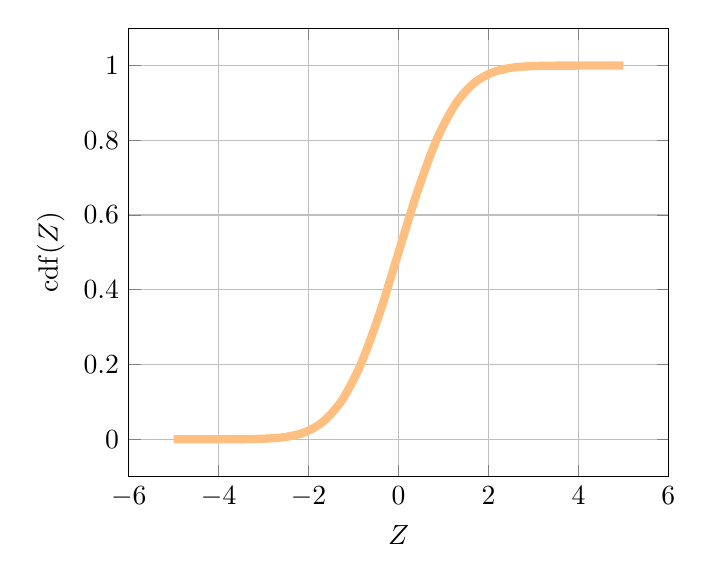
\begin{tikzpicture}
\begin{axis}[%
  xlabel=$Z$,
  ylabel=$\CDF(Z)$,
  grid=major,
 % legend entries={gnuplot, Bowling et al},
  legend pos=south east]
%  \addplot[smooth, line width=5pt, orange!50] gnuplot{\cdf(x)(0)(2)};
  \addplot [smooth, line width=3pt, orange!50] {normcdf(x,0,1)};
\end{axis}
\end{tikzpicture}
\end{frame}
\section{Odds ratio}
\begin{frame}{Odds ratio}
\begin{itemize}
\item logistic function: \[F(Y)=\text{log} \frac{P_{i}}{1-P_{i}}=exp(\eta) \]
\[ \eta \equiv \sum \beta_{k}X_{ik}\]
\item 為何logit做為一個連結函數,會產生$\{-\infty, \infty \}$的對應值?這是因為logit的函數是一個勝算比的型態。
\item Odds ratio(OR, 勝算比) 等於$\frac{P}{(1-P)}$。P、1-P、OR三者有以下的關係:
\begin{table}
\begin{center}
\begin{tabular}{| r | r | r | r | r | r |}
\hline
P & 0 & $\frac{1}{4}$ &  $\frac{1}{2}$ & $\frac{3}{4}$ & 1 \\
\hline
1-P & 1 & $\frac{3}{4}$ & $\frac{1}{2}$ & $\frac{1}{4}$ & 0 \\
\hline
OR & 0 & $\frac{1}{3}$ & 1 & 3 & $\infty$ \\
\hline
\end{tabular}
\end{center}
\end{table}
\item 對OR取對數,也就是log$(\frac{P_{i}}{1-P_{i}})$,ln(OR)範圍是$\{-\infty, \infty \}$
\item 因此,logit(Y)轉化為log$\frac{P}{1-P}$
\item logistic 與 probit模型的機率密度非常接近,得到的結果類似。
\end{itemize}
\end{frame}
\begin{frame}{勝算對數與模型}
\begin{itemize}
\item 定義$\Omega_{i}=\frac{P_{i}}{1-P_{i}}$,ln$\Omega_{i}$=ln$\frac{P_{i}}{1-P_{i}}$
\item 當勝算($\frac{P_{i}}{1-P_{i}}$)>1,勝算對數ln$\Omega_{i}>0$。
\item 當$0<\frac{P_{i}}{1-P_{i}}<1$,勝算對數ln$\Omega_{i}<0$。
\item 當$\frac{P_{i}}{1-P_{i}}=1$,勝算對數ln$\Omega_{i}=0$。
\item 勝算對數模型可寫成
\[\text{ln}\mathlarger{\frac{P}{1-P}}=X\beta \]
\item 經過運算,可寫成
\[\text{Pr}(y=1|\bf{x})=\frac{exp(\bf{x\beta})}{1+exp(\bf{x\beta})}\]
\item \textbf{x$\beta$}表示有一連串的x以及$\beta$
\end{itemize}
\end{frame}
\subsection{勝算對數模型實例}
\begin{frame}{勝算對數模型實例}
\begin{itemize}
\item 假設有一個自變數的值為1到5,估計logit模型得到ln$\frac{P_{i}}{1-P_{i}}=1+0.5X$
\item 當x=1,exp(x$\beta$)=exp(1.5)=4.48,而1+exp(3.5)=5.48,Pr(y=1|x=1)=$\frac{4.48}{5.48}$=0.81
\item 當x=2,Pr(y=1|x=2)=0.88
\item 當x=3,Pr(y=1|x=3)=0.92
\item 可以看出當x增加1個單位,機率增加的程度會因為x從哪一個值增加而有所不同。
\item 但是exp($\beta$)= exp(0.5)=1.64,表示增加勝算1.64-1=64\%。增加勝算的幅度是固定的,並不會因為x的大小而不同。
\item 而exp($\beta$)= exp(0.5)=1.64,表示x每增加1個單位,y是1對上y是0的勝算比,或者是勝算的對數(log of odds)增加1.64。
\end{itemize}
\end{frame}
\subsection{隱性模型}
\begin{frame}{隱性模型}
\begin{itemize}
\item 有學者從二元變數y為觀察值,但是$y^{*}$為觀察不到的隱性變數說明機率模型,而且
\[ y_{i}^{*}=\bf{x}_{i}\beta + \epsilon_{i}\]
\item $y^{*}$和$y_{i} $兩者之間的關係可表示為:
\begin{align*}
 y_{i} &=
  \begin{cases}
   0        & \text{if }\hspace{1em}  y_{i}^{*} \leq \tau \\
   1        & \text{if}\hspace{1em} y_{i}^{*} > \tau
  \end{cases}
 \end{align*}
\item $\tau$稱為「門檻」(threshold) 或是「截點 」(cutpoint)。在二元變數的模型,可以假定$\tau=0$
\item 由於$y_{i}^{*}$是無法觀察的變數,因此必須要用最大概似法加以估計。而在估計前須假設誤差項$\epsilon$的分佈,
\begin{enumerate}
\item 「機率單元模型」假設$\epsilon\sim N(0, 1)$
\item 「勝算對數模型」假設$\epsilon\sim N(0, \pi^2/3)$,其中$\pi^2/3\approx 3.29$
\end{enumerate}
\item 以上的兩種模型可以統一表示為Pr(y=1|x)=F(x$\beta$),F($\cdot$)可以是常態分佈的累積機率密度$\Phi$,或是logistic累積機率密度$\Lambda$
\end{itemize}
\end{frame}
\section{模型估計}
\begin{frame}{最大概似法}
\begin{itemize}
\item 最大概似法(Maximum Likelihood Estimation, MLE)的原理是對每一組$(x_{i}, y_{i})$,嘗試Pr($y_{i}=1$)=$\Phi(\text{X}\beta)$之中的$\beta$值,最大化出現Pr($y_{i}=1$)的機率。
\item 例如我們嘗試$\beta$值得到Pr($y_{i}=1$)=0.8,而且實際上$y_{i}=1$,我們可以說得到的概似機率為0.8。如果實際上$y_{i}=0$,我們可以說得到的概似機率為0.2。
\item 我們用$\mathcal{L}(y_{i}|\beta)$代表有$\beta$的條件下的$y_{i}$的概似機率,如果連乘所有的機率$\mathcal{L}(y_{1})\mathcal{L}(y_{2})\cdot\ldots\cdot\mathcal{L}(y_{n})=\prod_{i=1}^n\mathcal{L}(y_{i})$
\begin{align}
\text{max}\sum_{i=1}^{n}[\text{log}\mathcal{L}(y_{i}|\hat{\pi})]&=\sum \text{log}[\hat{\pi}^{y_{i}}(1-\hat{\pi})^{1-y_{i}}] \nonumber \\
  & =  \sum y_{i}\text{log}(\hat{\pi})+(1-y_{i})\text{log}(1-\hat{\pi})
\label{eq:max}
\end{align}
\item 對方程式\hspace{.5em}\textcolor{white}{\ref{eq:max}}\hspace{.5em}的$\hat{\pi}$取微分,並且設為0求出$\hat{\pi}$
\[\pi=\mathlarger{\frac{\sum_{i=1}^n y_{i}}{n}} \]
\end{itemize}
\end{frame}
\begin{frame}{MLE}
\begin{itemize} 
\item MLE的過程,需要使用Talyor series,讓概似機率逼近真實的機率。
\item 概似機率的估計式的抽樣分佈會接近常態分佈,N(0, H),其中H代表Hessian matrix (海森矩陣)
\item $\hat{\pi}=\mathlarger{\frac{\sum_{i=1}^n y_{i}}{n}}$表示樣本平均數可以最大化概似函數。
\item 將$\hat{\pi}$代入$\pi=\mathlarger{\frac{1}{1+exp{-X\beta}}}$,應用重複加權(iteratively reweighted least squares (IRLS))的演算式,聚合以下算式:
\[\hat{\beta}=\mathlarger{(X^{T}WX)^{-1}X^{T}Wz} \]
\item 進一步計算$\beta$的標準誤,表示為:
\[\hat{\beta}\sim \mathlarger{N(\beta, \phi(X^{T}WX)^{-1})} \]
\end{itemize}
\end{frame}

\begin{frame}{MLE的應用}
\begin{itemize} 
%\item MLE的過程,需要使用Talyor series,讓概似機率逼近真實的機率。
%\item 概似機率的估計式的抽樣分佈會接近常態分佈,N(0, H),其中H代表Hessian matrix (海森矩陣)
\item MLE也適用在線性迴歸,見Gary King (1989) \textit{Unifying Political Methodology}
\item 貝氏統計也需要MLE構成可觀察資料的模型,乘以先驗的資訊得到後驗的機率分佈。
\end{itemize}
\end{frame}
\section{信賴區間}
\begin{frame}{信賴區間}
\begin{itemize} 
\item 當依變數$y_{i}\hspace{.5em}\sim\hspace{.5em} \text{Bin}(1,\pi_{i})$,logit 模型可寫成:
\begin{equation}
\text{ln}\mathlarger{\frac{\pi_{i}}{1-\pi_{i}}}=X\beta 
\end{equation}
\item 或者是 logistic 迴歸模型:
\begin{equation}
\pi_{i}=\mathlarger{\frac{exp(X\beta)}{1+exp(X\beta)}} 
\end{equation}
\item 應用重複加權(IRLS)的演算式,計算$\widehat{SE}$,得到上下區間:
\[ \mathlarger{(\hat{\pi}-z_{\alpha/2}\widehat{SE},\hspace{1em}\hat{\pi}+z_{\alpha/2}\widehat{SE})} \]
\item 而且
\[\mathlarger{\frac{\hat{\beta_{j}} - \beta_{j}}{\widehat{SE}}}\sim z \]
\item 其中,$\widehat{SE}=\mathlarger{\sqrt{x^{T}(X{T}WX)^{-1}x)}}$
\end{itemize}
\end{frame}
\begin{frame}{運用IRLS}
\begin{itemize}
\item 運用IRLS 可以得到與\texttt{R}一樣的估計
\item 特別注意要去掉遺漏值
\item 見Patrick Breheny的語法:\url{http://web.as.uky.edu/statistics/users/pbreheny/760/S13/notes/2-21.R}
\end{itemize}
\end{frame}
\subsection{假設檢定}
\begin{frame}{假設檢定}
\begin{itemize} 
\item 理論上可以檢定$\textit{H}_{0}$:\hspace{.6em}$\pi=\pi_{0}$,根據這項假設計算$x\beta$
\item 但是實際上我們直接計算區間估計,判斷是否顯著不等於0。
\item 區間估計分為Wald 與 Likelihood ratio兩種
\end{itemize}
\end{frame}

\subsection{Wald test}
\begin{frame}{Wald test}
\begin{itemize} 
\item Abraham Wald 依據MLE發展出Wald confidence intervals, Wald test statistics等等
\item Wald 的方法依賴對於概似機率的趨近,如果概似機率不佳,也就是$\hat{\beta}$與$\beta$相差很大,Wald的檢定結果就會不夠好
\end{itemize}
\end{frame}
\subsection{LR test}
\begin{frame}{Likelihood ratio (LR) test}
\begin{itemize} 
\item LR 檢定的原理是比較兩個模型,一個是具有所有資訊(以$\theta$表示)的模型,一個是具有部分資訊(以$\hat{\theta}$表示)的模型。這兩個模型的比例表示為
\[\lambda=\frac{\mathcal{L}(\theta)}{\mathcal{L}(\hat{\theta})} \]
\begin{exampleblock}{定理}
當$n\longrightarrow \infty$,-2log$\lambda\hspace{.5em}\xrightarrow{d}\hspace{.5em}\chi^2$
\end{exampleblock}
\item 根據以上的定理,可導出
\[-2\text{log}\mathlarger\frac{L(\hat{\beta}|\beta^{1}=\beta^{1}_{0})}{L(\hat{\beta})}\leq \chi^2_{1-\alpha, q} \]
\item 其中$q$代表自由度,$\chi^2_{1-\alpha, q}$代表$\chi^2$分布的(1-$\alpha$)百分位
\end{itemize}
\end{frame}
\section{詮釋模型估計}
\begin{frame}{詮釋logit模型}
\begin{itemize} 
\item  logistic 迴歸模型:
\begin{equation}
\pi_{i}=\mathlarger{\frac{exp(X\beta)}{1+exp(X\beta)}} 
\end{equation}
\item 求出$\beta$之後,代入資料中的觀察值,可計算$\hat{\pi}=\frac{exp^{\eta}}{1+exp^{\eta}}$
\item 其中$\eta=X\beta$
\item 也可以說明X增加一個單位時,勝算對數比增加$exp(\beta)$倍
\end{itemize}
\end{frame}
\begin{frame}{詮釋logit模型}
\begin{itemize} 
\item  logistic 迴歸模型:
\begin{equation}
\pi_{i}=\mathlarger{\frac{exp(X\beta)}{1+exp(X\beta)}} 
\end{equation}
\item 或者是
\[\frac{\pi}{1-\pi}=exp(X\beta) \]
\item 如果$x_{1}$求出$\pi_{1}$,$x_{2}$對應$\pi_{2}$,這兩者的勝算比為
\[\mathlarger{\frac{\pi_{2}/(1-\pi_{2})}{\pi_{1}/(1-\pi_{1})}=\frac{exp(x_{2}\beta)}{exp(x_{1}\beta)}}=exp((x_{2}-x_{1})\beta) \]
\item 因此,當X增加$\delta$單位時,勝算對數比增加$exp(\delta\cdot\beta)$倍
\end{itemize}
\end{frame}
\section{軟體操作}
\subsection{SPSS}
\begin{frame}{實例}
\begin{itemize}
\item 以「認為住在一個民主國家重不重要1到10的程度」,預測「最近是否參加示威遊行」
\[ \text{Pr}(y=1|x)=\frac{exp(x\beta)}{1+exp(x\beta)} \]
\begin{align*}
y=\begin{cases}
1\hspace{1.2em}protest \\
0\hspace{1.2em}otherwise \\
\end{cases}
\end{align*}
\end{itemize}
\end{frame}
\begin{frame}{SPSS 程式與結果}
\begin{itemize}
\item SPSS程式
\begin{center}
\begin{figure}
\includegraphics[scale=0.5]{logit1.png}
\end{center}
\end{figure}
\end{itemize}
\end{frame}
\begin{frame}{SPSS 程式與結果}
\begin{itemize}
\item SPSS報表
\begin{center}
\begin{figure}
\includegraphics[scale=0.5]{logit2.png}
\end{center}
\end{figure}
\end{itemize}
\end{frame}
\subsection{Stata}
\begin{frame}{Stata 程式與結果}
\begin{itemize}
\item Stata 程式與結果
\begin{center}
\begin{figure}
\includegraphics[scale=0.5]{stata1.png}
\end{center}
\end{figure}
\end{itemize}
\end{frame}
\subsection{R}
\begin{frame}[fragile=singleslide]{R的logit迴歸模型程式}
\begin{Verbatim}[label=\textit{R code}, formatcom=\color{yellow}, frame=single]
> m1<-glm(protest ~ democracy, 
	           family=binomial(logit) )
> summary(m1)
\end{Verbatim}
\end{frame}
\begin{frame}[fragile=singleslide]{R 的logit迴歸模型估計結果}
\small
\begin{Verbatim}[label=\textit{R output}, formatcom=\color{yellow}, frame=single]
Call:
glm(formula = protest ~ democracy, 
                           family = binomial(logit))
Coefficients:
            Estimate Std. Error z value Pr(>|z|)    
(Intercept) -3.04362    0.36654  -8.304  < 2e-16 ***
democracy    0.15346    0.04301   3.568 0.000359 ***
---
Signif. codes:  0 ‘***’ 0.001 ‘**’ 0.01 ‘*’ 0.05 ‘.’ 0.1 ‘ ’ 1

(Dispersion parameter for binomial family taken to be 1)
    Null deviance: 1132.6  on 1383  degrees of freedom
Residual deviance: 1118.7  on 1382  degrees of freedom
  (33 observations deleted due to missingness)
AIC: 1122.7
\end{Verbatim}
\end{frame}
\begin{frame}[fragile=singleslide]{R 的probit迴歸模型估計結果}
\small
\begin{Verbatim}[label=\textit{R output}, formatcom=\color{yellow}, frame=single]
Call:
glm(formula = protest ~ democracy, 
                          family = binomial(probit))

Coefficients:
            Estimate Std. Error z value Pr(>|z|)    
(Intercept) -1.72079    0.18865  -9.122  < 2e-16 ***
democracy    0.08047    0.02246   3.582  0.00034 ***
---
Signif. codes:  0 ‘***’ 0.001 ‘**’ 0.01 ‘*’ 0.05 ‘.’ 0.1 ‘ ’ 1
(Dispersion parameter for binomial family taken to be 1)

    Null deviance: 1132.6  on 1383  degrees of freedom
Residual deviance: 1118.9  on 1382  degrees of freedom
  (33 observations deleted due to missingness)
AIC: 1122.9
\end{Verbatim}
\end{frame}
\subsection{多變數logistic迴歸模型}
\begin{frame}[fragile=singleslide]{多變數logistic迴歸模型}
\small
\begin{Verbatim}[label=\textit{R code}, formatcom=\color{yellow}, frame=single]
donner <- read.delim("http://web.as.uky.edu
                      /statistics/users
                      /pbreheny/760
                     /data/donner.txt")
fit <- glm(Status~Age*Sex,data=donner,
                         family=binomial)
\end{Verbatim}
\end{frame}
\begin{frame}[fragile=singleslide]{多變數logistic迴歸模型}
\small
\begin{Verbatim}[label=\textit{R output}, formatcom=\color{yellow}, frame=single]
> summary(fit)
Call:
glm(formula = Status ~ Age * Sex, 
              family = binomial, data = donner)

Deviance Residuals: 
    Min       1Q   Median       3Q      Max  
-2.2279  -0.9388  -0.5550   0.7794   1.6998  

Coefficients:
            Estimate Std. Error z value Pr(>|z|)  
(Intercept)  7.24638    3.20517   2.261   0.0238 *
Age         -0.19407    0.08742  -2.220   0.0264 *
SexMale     -6.92805    3.39887  -2.038   0.0415 *
Age:SexMale  0.16160    0.09426   1.714   0.0865 .
---
Signif. codes:  0 ‘***’ 0.001 ‘**’ 0.01 ‘*’ 0.05 ‘.’ 0.1 ‘ ’ 1
(Dispersion parameter for binomial family taken to be 1)
    Null deviance: 61.827  on 44  degrees of freedom
Residual deviance: 47.346  on 41  degrees of freedom
AIC: 55.346
Number of Fisher Scoring iterations: 5
\end{Verbatim}
\end{frame}

\begin{frame}[fragile=singleslide]{多變數logistic迴歸模型}
\small
\begin{Verbatim}[label=\textit{R output}, formatcom=\color{yellow}, frame=single]
> confint(fit)          ## Likelihood ratio
                   2.5 %      97.5 %
(Intercept)   2.357779417 16.04184845
Age          -0.427958905 -0.05689585
SexMale     -15.925314742 -1.41347947
Age:SexMale   0.001308492  0.40260315
> confint.default(fit)  ## Wald
                   2.5 %      97.5 %
(Intercept)   0.96437239 13.52839716
Age          -0.36540516 -0.02274311
SexMale     -13.58971552 -0.26638343
Age:SexMale  -0.02315309  0.34634682
\end{Verbatim}
\end{frame}
\section{結論}
\begin{frame}{結論}
\normalsize
\begin{itemize}
\item 了解為什麼線性模型不適用於依變數為二元變數
\item 認識logit 與 probit 模型的基本原理
\item 了解如何估計logit 與 probit 模型
\item 了解如何詮釋logit  模型的係數與模型適合度
\end{itemize}
\end{frame}

\end{document}